\section{Parameter arrays, price plots, and surface dynamics}
\label{sec:figures}

All parameters and the full reset-diagnostics array are exported by
\texttt{report/generate\_report\_artifacts.py} to
\texttt{report/data/parameters.json}, reproduced exactly from the
manuscript's own synthetic sequence (Table~\ref{tab:params}).

\begin{table}[H]
\centering
\small
\begin{tabular}{ll}
\toprule
Parameter & Value \\
\midrule
$T_*$ & $20/252$ \\
Reset times $(t_1,t_2,t_3)$ & $(2,7,12)/252$ \\
Model expiries & $(5,10,15,20)/252$ \\
$(Y_0,V_0,\kappa,\xi,\rho)$ & $(1,\,0.04,\,2,\,0.30,\,-0.70)$ \\
$\theta_0$, $[\theta_{\min},\theta_{\max}]$ & $0.040$, $[0.025,0.055]$ \\
$(r_1,r_2,r_3)$ & $(0.006,0.006,0.006)$ \\
$(\Lambda,M,\delta_{\min},\delta_{\max},s_*)$ & $(0.5,\,0.05,\,0.08,\,0.15,\,0.25)$ \\
\bottomrule
\end{tabular}
\caption{The manuscript's own fully-specified synthetic reset sequence, reproduced exactly.}
\label{tab:params}
\end{table}

\begin{figure}[H]
\centering
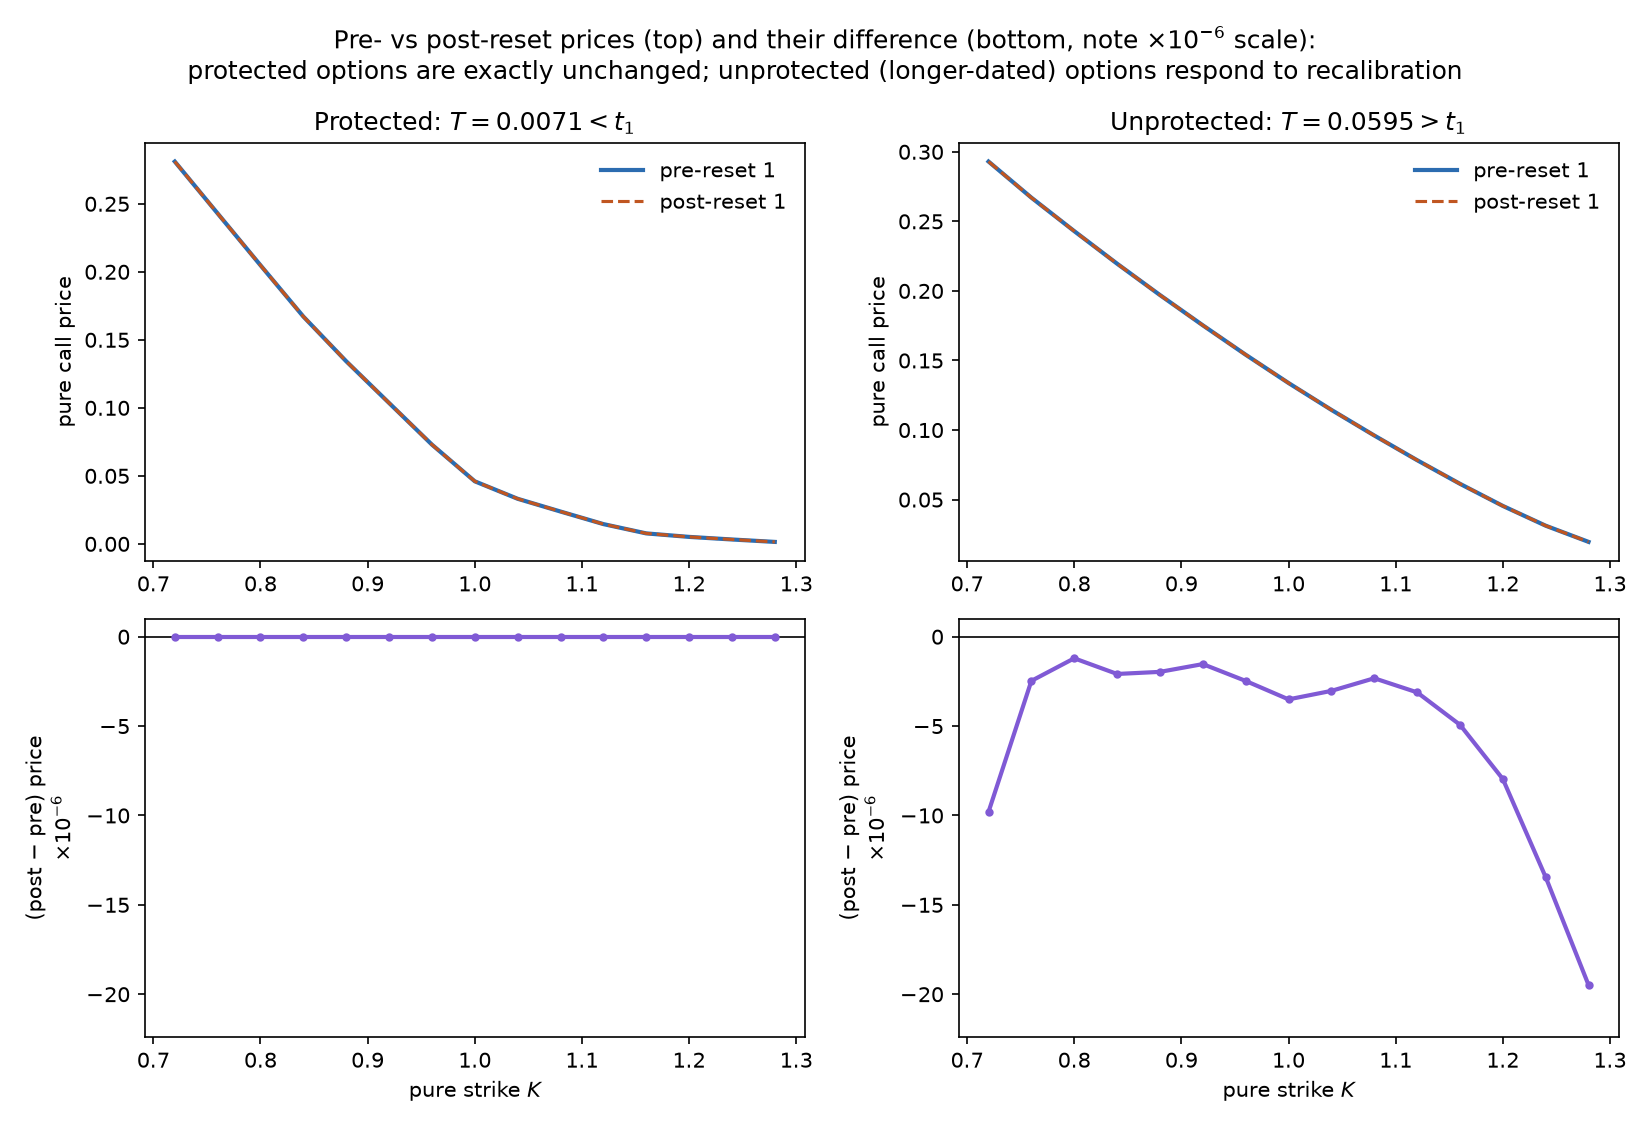
\includegraphics[width=\textwidth]{figures/protected_vs_unprotected.png}
\caption{Pre- vs.\ post-reset-1 price curves across strike. Left: a
protected maturity ($T<t_1$) -- the two curves are numerically
indistinguishable. Right: an unprotected maturity ($T>t_1$) -- the curves
differ, reflecting the recalibration's intended effect on longer-dated
options.}
\label{fig:protected-vs-unprotected}
\end{figure}

\begin{figure}[H]
\centering
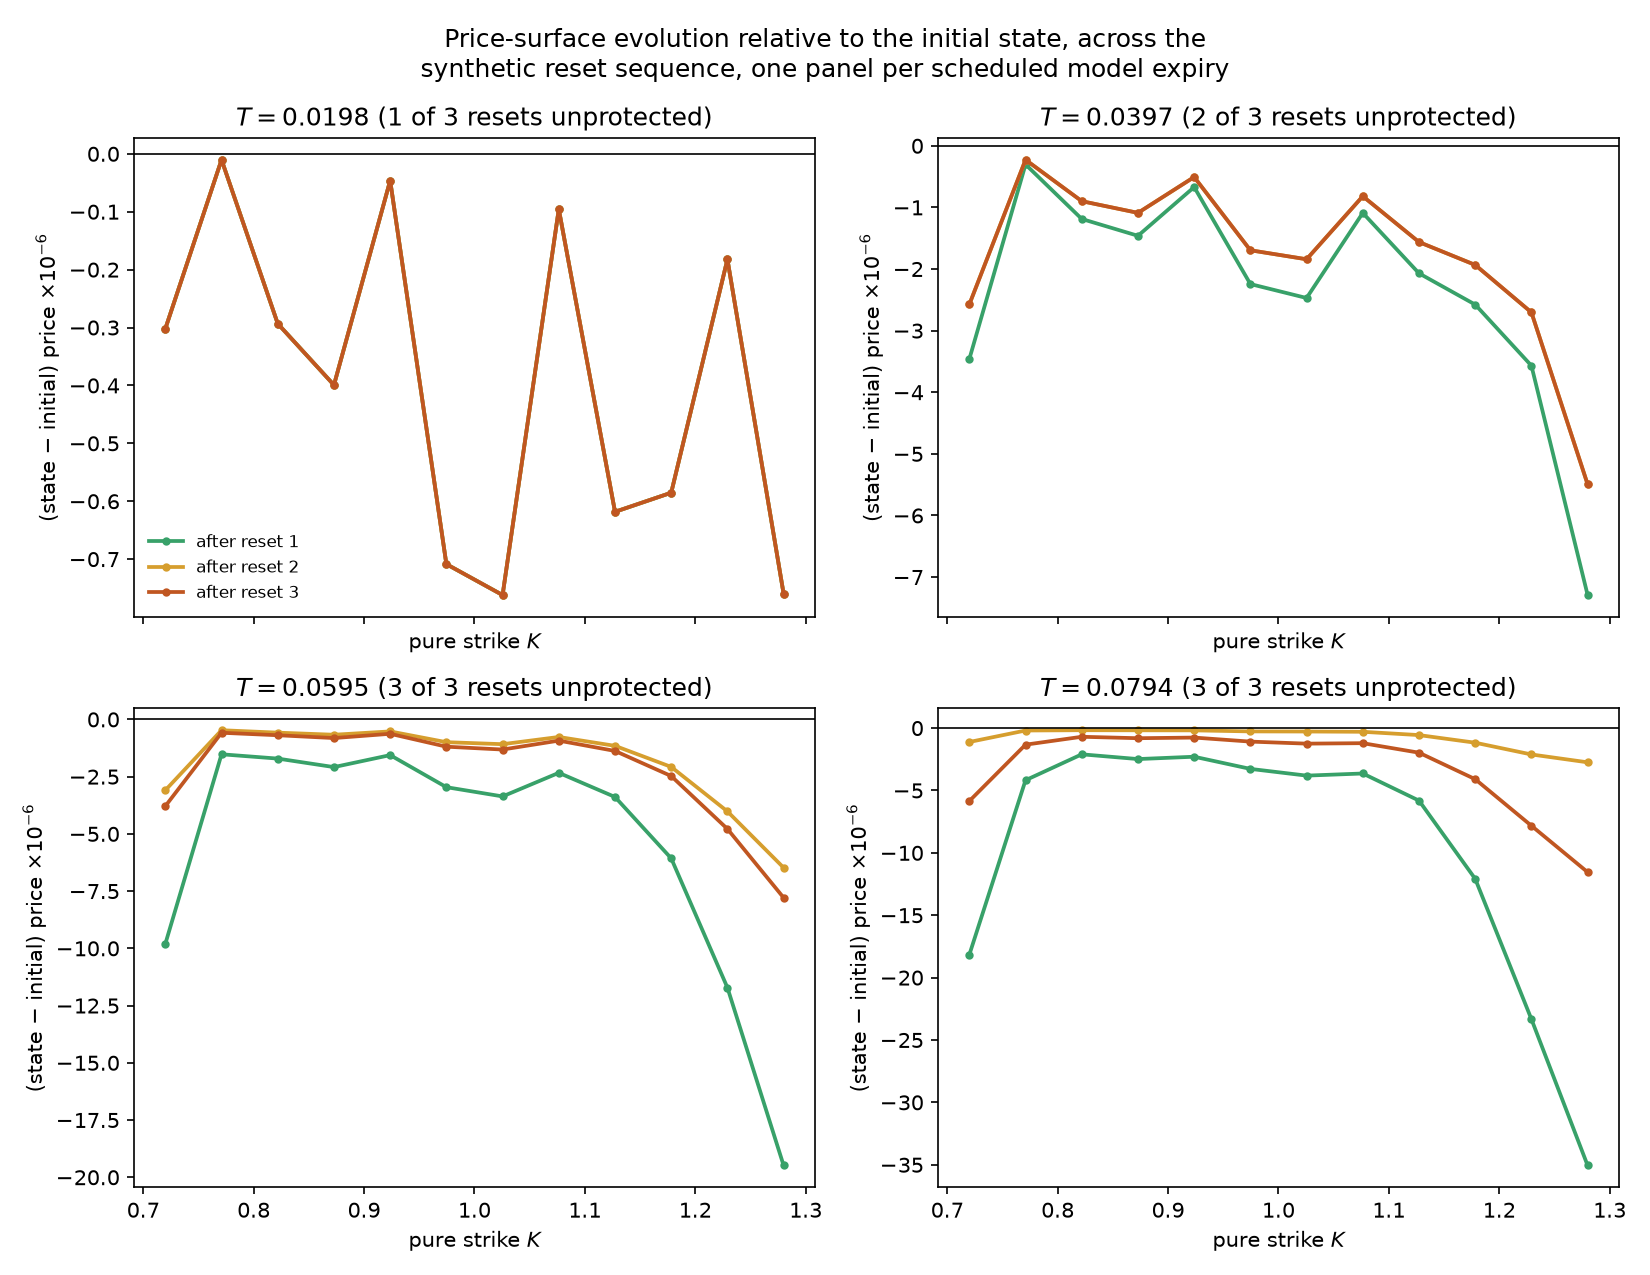
\includegraphics[width=\textwidth]{figures/surface_dynamics.png}
\caption{Price DIFFERENCE from the initial state (note $10^{-6}$ scale), at
each of the four scheduled model expiries, one line per post-reset state.
As required, the ``after reset 2'' and ``after reset 3'' curves coincide
exactly with ``after reset 1'' whenever $T$ is still protected relative to
resets 2/3 (top-left and top-right panels), and separate once $T$ passes
those reset times (bottom row) -- confirming the same protected/unprotected
structure as Fig.~\ref{fig:protected-vs-unprotected} across the whole
surface. The top-left panel's exact shape is numerically delicate (its
signal, $\lesssim10^{-6}$ in absolute price, sits close to this
maturity's Fourier-quadrature floor at the settings used for this plot) --
its curves coinciding is reliable, but its precise zigzag shape should not
be over-interpreted.}
\label{fig:surface-dynamics}
\end{figure}
